% ============================================================
%  S3 -- Estatística Aplicada ao Mercado Financeiro
%  Núcleo Quant · Liga de Mercado Financeiro · UFU · 2026.1
%  Estudo Guiado -- Aula Assíncrona
% ============================================================
\documentclass[11pt,a4paper]{article}

% ─── Pacotes ────────────────────────────────────────────────────────────────
\usepackage[utf8]{inputenc}
\usepackage[T1]{fontenc}
\usepackage[top=3.5cm, bottom=2.5cm, left=2.5cm, right=2.5cm]{geometry}
\usepackage{xcolor}
\usepackage{titlesec}
\usepackage{enumitem}
\usepackage{amsmath, amssymb, amsthm, mathtools}
\usepackage{graphicx}
\usepackage{fancyhdr}
\usepackage{tcolorbox}
\usepackage{tabularx}
\usepackage{booktabs}
\usepackage{array}
\usepackage{float}
\usepackage{tikz}
\usepackage{pgfplots}
\pgfplotsset{compat=1.18}
\usepackage{hyperref}
\usepackage{csquotes}
\usepackage{setspace}

\tcbuselibrary{skins, breakable}
\usetikzlibrary{arrows.meta, positioning}

% ─── Cores ──────────────────────────────────────────────────────────────────
\definecolor{quantpurple}{HTML}{7B2FBE}
\definecolor{quantpurplelight}{HTML}{F0E8FF}
\definecolor{quantdark}{HTML}{1A1A1A}
\definecolor{quantgray}{HTML}{6B7280}
\definecolor{quantlightgray}{HTML}{F3F4F6}
\definecolor{quantgreen}{HTML}{16A34A}
\definecolor{quantred}{HTML}{DC2626}
\definecolor{quantamber}{HTML}{D97706}
\definecolor{quantblue}{HTML}{1D4ED8}
\definecolor{quantbluelight}{HTML}{EFF6FF}
\definecolor{colnormal}{HTML}{2196F3}
\definecolor{colt}{HTML}{E53935}

% ─── Fonte: sans-serif em todo o documento ───────────────────────────────────
\renewcommand{\familydefault}{\sfdefault}

% ─── Hyperlinks ─────────────────────────────────────────────────────────────
\hypersetup{hidelinks}

% ─── Espaçamento de parágrafos ───────────────────────────────────────────────
\setlength{\parskip}{4pt}
\setlength{\parindent}{0pt}

% ─── Cabeçalho e rodapé ─────────────────────────────────────────────────────
\setlength{\headheight}{2cm}
\setlength{\headsep}{1cm}

\pagestyle{fancy}
\fancyhf{}
\renewcommand{\headrulewidth}{0pt}
\fancyhead[L]{%
  
\includegraphics[height=1.40cm]{logoSimples.png}%
}
\fancyhead[R]{%
  \raisebox{0.5cm}{\textcolor{quantgray}{\footnotesize
    Núcleo Quant
    \,$\cdot$\, Liga de Mercado Financeiro
    \,$\cdot$\, UFU \,$\cdot$\, 2026.1}}%
}
\fancyfoot[C]{\textcolor{quantgray}{\footnotesize\thepage}}
\fancyfoot[R]{%
  \textcolor{quantgray}{\footnotesize
    Aula S3 \,$\cdot$\, Estatística Aplicada ao Mercado Financeiro}%
}

% ─── Títulos de seção ───────────────────────────────────────────────────────
\titleformat{\section}
  {\large\bfseries\sffamily\color{quantpurple}}
  {}{0em}{}
  [\vspace{2pt}\textcolor{quantpurple}{\rule{\textwidth}{1.2pt}}\vspace{4pt}]

\titleformat{\subsection}
  {\normalsize\bfseries\sffamily\color{quantdark}}
  {}{0em}{}

\titlespacing{\section}{0pt}{20pt}{6pt}
\titlespacing{\subsection}{0pt}{14pt}{4pt}

% ─── Listas ─────────────────────────────────────────────────────────────────
\setlist[itemize]{
  label=\textcolor{quantpurple}{\small$\blacktriangleright$},
  leftmargin=1.8em,
  itemsep=3pt,
  parsep=0pt
}
\setlist[enumerate]{
  label=\textcolor{quantpurple}{\textbf{\arabic*.}},
  leftmargin=1.8em,
  itemsep=5pt,
  parsep=0pt
}

% ─── Código inline ──────────────────────────────────────────────────────────
\newcommand{\code}[1]{%
  \colorbox{quantlightgray}{\texttt{\small\color{quantdark}#1}}%
}

% ─── Comandos matemáticos ───────────────────────────────────────────────────
\newcommand{\E}{\mathbb{E}}
\newcommand{\Var}{\mathrm{Var}}
\newcommand{\Cov}{\mathrm{Cov}}

% ─── Teoremas: fonte sans-serif, mesmo tamanho do corpo ─────────────────────
\newtheoremstyle{quant}%
  {8pt}{6pt}%            espaço acima e abaixo
  {\normalfont\sffamily}%  fonte do corpo
  {}%                    recuo
  {\bfseries\sffamily}%  fonte do título
  {.}%                   pontuação após título
  { }%                   espaço após título
  {}%                    especificação de cabeçalho

\theoremstyle{quant}
\newtheorem{definicao}{Definição}[section]
\newtheorem{exemplo}{Exemplo}[section]
\newtheorem{propriedade}{Propriedade}[section]

% ─── Caixa de destaque (roxo claro) ─────────────────────────────────────────
\newtcolorbox{highlightbox}{
  enhanced,
  colback=quantpurplelight,
  colframe=quantpurple,
  boxrule=1pt,
  arc=4pt,
  left=10pt, right=10pt, top=7pt, bottom=7pt,
  fontupper=\small\sffamily\color{quantdark}
}

% ─── Caixa de script Python ─────────────────────────────────────────────────
\newtcolorbox{caixapy}[1]{
  enhanced,
  colback=white,
  colframe=quantpurple,
  boxrule=0.8pt,
  arc=4pt,
  title={\textbf{\textcolor{white}{\small\sffamily Script Python: \texttt{#1}}}},
  attach boxed title to top left={yshift=-1mm, xshift=10pt},
  boxed title style={
    colback=quantpurple, colframe=quantpurple,
    arc=3pt, boxrule=0pt,
    left=6pt, right=6pt, top=2pt, bottom=2pt
  },
  left=10pt, right=10pt, top=14pt, bottom=8pt,
  fontupper=\small\sffamily\color{quantdark},
  breakable,
}

% ─── Caixa de insight financeiro (azul) ─────────────────────────────────────
\newtcolorbox{caixainsight}{
  enhanced,
  colback=quantbluelight,
  colframe=quantblue,
  boxrule=0.8pt,
  arc=4pt,
  title={\textbf{\textcolor{white}{\small\sffamily Insight Financeiro}}},
  attach boxed title to top left={yshift=-1mm, xshift=10pt},
  boxed title style={
    colback=quantblue, colframe=quantblue,
    arc=3pt, boxrule=0pt,
    left=6pt, right=6pt, top=2pt, bottom=2pt
  },
  left=10pt, right=10pt, top=14pt, bottom=8pt,
  fontupper=\small\sffamily\color{quantdark},
  breakable,
}

% ─── Caixa de atenção (âmbar) ───────────────────────────────────────────────
\newtcolorbox{caixaatencao}{
  enhanced,
  colback=white,
  colframe=quantamber,
  boxrule=0.8pt,
  arc=4pt,
  title={\textbf{\textcolor{white}{\small\sffamily Atenção}}},
  attach boxed title to top left={yshift=-1mm, xshift=10pt},
  boxed title style={
    colback=quantamber, colframe=quantamber,
    arc=3pt, boxrule=0pt,
    left=6pt, right=6pt, top=2pt, bottom=2pt
  },
  left=10pt, right=10pt, top=14pt, bottom=8pt,
  fontupper=\small\sffamily\color{quantdark},
}

% ─── Caixa de resumo (verde) ────────────────────────────────────────────────
\newtcolorbox{caixaresumo}{
  enhanced,
  colback=white,
  colframe=quantgreen,
  boxrule=0.8pt,
  arc=4pt,
  title={\textbf{\textcolor{white}{\small\sffamily Resumo do Tópico}}},
  attach boxed title to top left={yshift=-1mm, xshift=10pt},
  boxed title style={
    colback=quantgreen, colframe=quantgreen,
    arc=3pt, boxrule=0pt,
    left=6pt, right=6pt, top=2pt, bottom=2pt
  },
  left=10pt, right=10pt, top=14pt, bottom=8pt,
  fontupper=\small\sffamily\color{quantdark},
  breakable,
}

% ════════════════════════════════════════════════════════════════════════════
\begin{document}
% ════════════════════════════════════════════════════════════════════════════

\thispagestyle{fancy}

% ─── Título ─────────────────────────────────────────────────────────────────
\begin{center}
  
\includegraphics[height=3cm]{logoLiga.png}\\[1em]
  {\fontsize{22}{26}\selectfont\bfseries\sffamily ESTUDO GUIADO -- S3}\\[0.4em]
  {\large\sffamily\textcolor{quantgray}{Estatística Aplicada ao Mercado Financeiro}}
\end{center}

\vspace{0.5em}
\textcolor{quantpurple}{\rule{\textwidth}{2pt}}
\vspace{1em}

% ─── Informações da aula ────────────────────────────────────────────────────
\begin{tabularx}{\textwidth}{@{}llX@{}}
  \toprule
  \textcolor{quantpurple}{\textbf{Bloco}} &
  \textcolor{quantpurple}{\textbf{Sessão}} &
  \textcolor{quantpurple}{\textbf{Formato}} \\
  \midrule
  Bloco 1 -- Fundamentos & S3 & Assíncrono (estudo individual) \\
  \bottomrule
\end{tabularx}

\vspace{0.8em}

\textbf{Pré-requisito:}\quad S1 e S2 (Python, pandas, retornos simples e log-retornos)

\vspace{0.5em}
\textbf{Scripts desta aula:}

\vspace{0.3em}
\begin{tabularx}{\textwidth}{@{}llX@{}}
  \toprule
  \textcolor{quantpurple}{\textbf{Arquivo}} &
  \textcolor{quantpurple}{\textbf{Tópico}} &
  \textcolor{quantpurple}{\textbf{Caso prático}} \\
  \midrule
  \code{s3\_01\_estatistica\_descritiva.py} & Estatística Descritiva & PETR4, VALE3 e ITUB4 (2020--2024) \\[3pt]
  \code{s3\_02\_distribuicoes.py}           & Distribuições          & IBOVESPA, VaR por distribuição \\[3pt]
  \code{s3\_03\_testes\_hipotese.py}        & Testes de Hipótese     & Retorno médio e autocorrelação \\[3pt]
  \code{s3\_04\_correlacao.py}              & Correlação             & Portfólio com 6 ativos \\
  \bottomrule
\end{tabularx}

\vspace{1em}

\begin{highlightbox}
  \textbf{Como usar este material:} leia cada seção e execute o script correspondente
  em paralelo. As caixas \textbf{Script Python} no início de cada seção indicam qual
  arquivo abrir. Instale as dependências com:\\[4pt]
  \code{pip install yfinance pandas numpy scipy statsmodels matplotlib seaborn}
\end{highlightbox}

\vspace{1.2em}
\textcolor{quantpurple}{\rule{\textwidth}{1.2pt}}

\newpage

% ─── Sumário ────────────────────────────────────────────────────────────────
\renewcommand{\contentsname}{Sumário}
\tableofcontents

\newpage

% ════════════════════════════════════════════════════════════════════════════
\section{Estatística Descritiva}
\label{sec:descritiva}
% ════════════════════════════════════════════════════════════════════════════

\begin{caixapy}{s3\_01\_estatistica\_descritiva.py}
  Caso prático: análise descritiva completa dos retornos diários de PETR4, VALE3 e ITUB4
  (2020--2024). Gera histogramas, boxplots e Q-Q plots comparativos.
  Execute este arquivo enquanto estuda esta seção.
\end{caixapy}

\subsection{Por que estatística descritiva em finanças?}

Antes de qualquer modelo (VaR, backtest, ML) precisamos \emph{entender} os dados.
A estatística descritiva resume uma série de números em poucas medidas essenciais,
respondendo a três perguntas fundamentais:

\begin{itemize}
  \item \textbf{Onde está o centro?} Quanto o ativo retorna em média?
  \item \textbf{Quão dispersos são os valores?} Qual a volatilidade?
  \item \textbf{Que formato tem a distribuição?} Os retornos são simétricos? Há eventos extremos frequentes?
\end{itemize}

Respostas erradas aqui se propagam para todo o pipeline quantitativo.
Um modelo de risco calibrado com a volatilidade errada subestima ou superestima
reservas de capital, com consequências reais.

\subsection{Medidas de Tendência Central}

\textbf{Tendência central} é o valor em torno do qual os retornos se concentram.

\begin{definicao}[Média Aritmética]
Dado um conjunto de $n$ retornos observados $r_1, r_2, \ldots, r_n$:
\[
  \bar{r} = \frac{1}{n}\sum_{i=1}^{n} r_i
\]
onde $r_i$ é o retorno do pregão $i$ e $n$ é o número total de observações.
A média considera todos os valores com peso igual, o que a torna sensível a
retornos extremos (crashes e rallies pontuais).
\end{definicao}

\begin{definicao}[Mediana]
A mediana $m$ é o valor que divide a amostra ao meio: exatamente metade dos
retornos fica abaixo dela e metade acima. Ao contrário da média, a mediana
\textbf{não é afetada por valores extremos}, pois depende apenas da posição
central dos dados, não de seus valores absolutos.

Em séries financeiras, compare sempre média e mediana:
\begin{itemize}
  \item $\bar{r} < m$: perdas extremas são mais intensas que ganhos extremos (assimétrico à esquerda)
  \item $\bar{r} > m$: ganhos extremos dominam (assimétrico à direita)
  \item $\bar{r} \approx m$: distribuição aproximadamente simétrica
\end{itemize}
\end{definicao}

\begin{definicao}[Retorno Médio Anualizado]
O Brasil usa 252 dias úteis como convenção anual. Dado o retorno médio diário
$\bar{r}_d$ calculado a partir de log-retornos:
\[
  \bar{r}_{\text{anual}} = \bar{r}_d \times 252
\]
Para retornos simples (calculados com \code{pct\_change()}), a anualização
correta é geométrica, pois os retornos se compõem multiplicativamente ao longo do tempo:
\[
  \bar{r}_{\text{anual}}^{\text{simples}} = (1 + \bar{r}_d)^{252} - 1
\]
\end{definicao}

\begin{caixainsight}
Para PETR4, a média dos retornos diários costuma ser menor que a mediana,
confirmando a assimetria esquerda típica de ações de alta volatilidade.
A maioria dos dias apresenta retorno ligeiramente positivo, mas os dias de queda
extrema são mais intensos, puxando a média para baixo. Esse padrão é a regra,
não a exceção, em ações brasileiras.
\end{caixainsight}

\subsection{Medidas de Dispersão}

\textbf{Dispersão} mede o quanto os retornos se afastam do valor central.
Em finanças, dispersão é sinônimo de \textbf{risco}: quanto mais dispersos os
retornos, mais incerto é o resultado futuro do investimento.

\begin{definicao}[Variância e Desvio-Padrão Amostral]
A \textbf{variância} mede a dispersão média ao quadrado em relação à média:
\[
  s^2 = \frac{1}{n-1}\sum_{i=1}^{n}(r_i - \bar{r})^2
\]
onde $r_i - \bar{r}$ é o desvio de cada retorno em relação à média, e $n-1$
(em vez de $n$) é a correção de Bessel, que torna $s^2$ um estimador não-enviesado
da variância populacional $\sigma^2$.

O \textbf{desvio-padrão} $s = \sqrt{s^2}$ tem a mesma unidade dos retornos
(por exemplo, \% ao dia) e é a medida de risco mais usada na prática.
\end{definicao}

\begin{definicao}[Volatilidade Anualizada]
A \textbf{volatilidade} é o desvio-padrão dos retornos, medida de risco padrão
da indústria. Para converter volatilidade diária em anual, usa-se a
\textbf{regra da raiz-quadrada do tempo}, válida quando os retornos de dias
diferentes são independentes entre si:
\[
  \sigma_{\text{anual}} = \sigma_{\text{diária}} \times \sqrt{252}
\]
Por exemplo, uma volatilidade diária $\sigma_{\text{diária}} = 1{,}5\%$ implica
volatilidade anual $\sigma_{\text{anual}} = 1{,}5\% \times \sqrt{252} \approx 23{,}8\%$.
\end{definicao}

\begin{caixaatencao}
A regra $\times\sqrt{252}$ pressupõe que os retornos de dias diferentes são
independentes. Quando há \textbf{agrupamento de volatilidade} (dias voláteis
tendem a ser seguidos por dias igualmente voláteis), essa regra subestima o
risco de longo prazo. Esse fenômeno é modelado pelos processos GARCH, vistos na S4.
\end{caixaatencao}

\begin{definicao}[Coeficiente de Variação (CV)]
O CV normaliza o risco pelo retorno, permitindo comparar ativos em escalas diferentes:
\[
  CV = \frac{\sigma}{|\bar{r}|}
\]
onde $\sigma$ é o desvio-padrão e $|\bar{r}|$ é o valor absoluto da média.
Um CV menor indica que o ativo entrega mais retorno por unidade de risco assumido.
\end{definicao}

\subsection{Quartis, IQR e Detecção de Outliers}

\textbf{Quartis} são pontos que dividem os dados ordenados em quatro partes iguais,
cada uma contendo 25\% das observações. Imagine todos os retornos do período
organizados do menor ao maior; os quartis marcam as posições 25\%, 50\% e 75\%
desse ordenamento:

\begin{definicao}[Quartis]
\begin{itemize}
  \item $Q_1$ (primeiro quartil): 25\% dos retornos ficam abaixo deste valor.
        É o percentil 25
  \item $Q_2$ (segundo quartil): a mediana. Exatamente metade dos retornos fica abaixo.
        É o percentil 50
  \item $Q_3$ (terceiro quartil): 75\% dos retornos ficam abaixo deste valor.
        É o percentil 75
\end{itemize}
A \textbf{Amplitude Interquartil (IQR)} é a distância entre o terceiro e o primeiro quartil:
\[
  \text{IQR} = Q_3 - Q_1
\]
O IQR representa a faixa central de 50\% dos retornos (do 25\textordmasculine\ ao 75\textordmasculine\ percentil),
ignorando os extremos de ambos os lados. Por isso é uma medida de dispersão
\textbf{robusta}: crashes e rallies pontuais não a afetam.
\end{definicao}

O critério de Tukey usa o IQR para identificar automaticamente retornos atípicos.
Uma observação é sinalizada como outlier se estiver fora do intervalo:
\[
  \bigl[Q_1 - 1{,}5\cdot\text{IQR},\;\; Q_3 + 1{,}5\cdot\text{IQR}\bigr]
\]
O boxplot visualiza exatamente essa estrutura: a caixa central abrange $Q_1$ a $Q_3$,
a linha interna é a mediana, e os pontos além dos limites são os outliers.

\subsection{Momentos Estatísticos: Assimetria e Curtose}

Média e desvio-padrão descrevem o centro e a dispersão, mas não dizem como os retornos
se distribuem em torno desse centro. Para isso, usamos dois \textbf{momentos} adicionais.

\textbf{O que é um momento estatístico?} É uma medida que resume uma característica
específica da forma de uma distribuição. A ideia vem da física: assim como o momento de
uma força captura sua intensidade e direção, cada momento estatístico captura um aspecto
diferente da distribuição. Calculamos os momentos elevando os desvios em relação à média
a potências sucessivas:

\begin{itemize}
  \item \textbf{1° momento} (média $\bar{r}$): descreve o \emph{centro} da distribuição.
        $\sum(r_i)/n$ -- os desvios elevados à 1ª potência
  \item \textbf{2° momento central} (variância $s^2$): descreve a \emph{dispersão}.
        $\sum(r_i - \bar{r})^2/n$ -- os desvios elevados ao quadrado, sempre positivos
  \item \textbf{3° momento padronizado} (assimetria $g_1$): descreve a \emph{direção}
        em que a distribuição inclina. O cubo preserva o sinal ($+$ ou $-$) do desvio,
        indicando se a cauda longa está à esquerda ou à direita
  \item \textbf{4° momento padronizado} (curtose $g_2$): descreve o \emph{peso das caudas}.
        A quarta potência amplifica desvios extremos muito mais do que desvios pequenos,
        capturando se os extremos são frequentes
\end{itemize}

\begin{definicao}[Assimetria (Skewness, $g_1$)]
A assimetria mede se a distribuição tem uma cauda mais longa de um lado.
É o terceiro momento padronizado:
\[
  g_1 = \frac{1}{n}\sum_{i=1}^{n}\left(\frac{r_i - \bar{r}}{s}\right)^{\!3}
\]
onde $r_i - \bar{r}$ é o desvio de cada retorno em relação à média e $s$ é o
desvio-padrão. A divisão por $s$ torna a medida adimensional (sem unidade),
comparável entre ativos diferentes. O expoente 3 preserva o sinal:
\begin{itemize}
  \item $g_1 = 0$: distribuição simétrica (caso da Normal)
  \item $g_1 < 0$: cauda esquerda mais longa; perdas extremas ocorrem com mais frequência
        ou magnitude do que ganhos extremos (\emph{negatively skewed})
  \item $g_1 > 0$: cauda direita mais longa; ganhos extremos dominam (\emph{positively skewed})
\end{itemize}
\end{definicao}

\begin{definicao}[Curtose e Curtose em Excesso ($g_2$, $\kappa$)]
A curtose mede o peso das caudas em relação à Normal.
É o quarto momento padronizado:
\[
  g_2 = \frac{1}{n}\sum_{i=1}^{n}\left(\frac{r_i - \bar{r}}{s}\right)^{\!4}
  \qquad \text{(curtose total)}
\]
O expoente 4 sempre resulta em valores positivos e amplifica desvios grandes,
tornando $g_2$ sensível a eventos extremos. A distribuição Normal tem
curtose total $g_2 = 3$. Subtrai-se 3 para obter a \textbf{curtose em excesso}
$\kappa$, que mede o excesso de peso nas caudas em relação à Normal:
\[
  \kappa = g_2 - 3
\]
\begin{itemize}
  \item $\kappa = 0$: caudas iguais à Normal (\emph{mesocúrtica})
  \item $\kappa > 0$: distribuição \textbf{leptocúrtica}; caudas mais pesadas, eventos extremos
        mais frequentes do que a Normal prevê
  \item $\kappa < 0$: distribuição \textbf{platicúrtica}; caudas mais leves, retornos
        concentrados próximos à média
\end{itemize}
\end{definicao}

\begin{caixainsight}
Ações do IBOVESPA tipicamente têm $g_1 < 0$ e $\kappa > 0$, combinação chamada de
\textbf{distribuição leptocúrtica assimétrica à esquerda}. A implicação para gestão de
risco é severa: modelos que assumem normalidade subestimam a probabilidade de perdas
extremas. Em 16 de março de 2020, o IBOVESPA caiu $-12{,}17\%$ em um único pregão.
Com $\sigma = 2\%$/dia, isso representa um evento de $-6{,}1\sigma$, ao qual a
distribuição Normal atribuiria probabilidade de $\approx 5{,}8 \times 10^{-10}$
(menos de 1 em 1 bilhão de pregões). Na prática, eventos assim ocorrem a cada
poucos anos.
\end{caixainsight}

\subsection{Percentis e o Value at Risk (VaR)}

Os \textbf{percentis} generalizam os quartis: onde os quartis dividem os dados em 4 partes,
os percentis permitem dividir em qualquer proporção. São especialmente importantes em
finanças porque os percentis inferiores correspondem às perdas extremas que definem o risco.

\begin{definicao}[Percentil]
O percentil $P_\alpha$ é o valor abaixo do qual se encontra exatamente $\alpha\%$
das observações. Para calculá-lo formalmente, precisamos da função de distribuição
acumulada (CDF), que para qualquer valor $x$ indica quantos por cento dos retornos
são menores que $x$:
\[
  F(x) = P(R \leq x) \qquad \text{(proporção de retornos menores que } x\text{)}
\]
O percentil $P_\alpha$ é o inverso dessa função: dado que queremos a proporção $\alpha/100$,
qual é o valor $x$ correspondente?
\[
  P_\alpha = F^{-1}\!\left(\frac{\alpha}{100}\right)
\]
\textbf{Exemplo prático:} $P_5 = F^{-1}(0{,}05)$ é o retorno abaixo do qual ficam
os piores 5\% dos dias. Se $P_5 = -2{,}8\%$, significa que em 5\% dos pregões
o ativo perdeu mais de 2,8\% em um único dia.
\end{definicao}

No contexto de risco, os percentis inferiores recebem o nome de \textbf{Value at Risk}:

\begin{itemize}
  \item $P_5 \Rightarrow$ \textbf{VaR 95\%}: perda que é excedida em apenas 5\% dos dias
  \item $P_1 \Rightarrow$ \textbf{VaR 99\%}: perda que é excedida em apenas 1\% dos dias
\end{itemize}

O VaR responde à pergunta: \emph{"qual é a pior perda esperada em condições normais de mercado?"}
Estudaremos o VaR em profundidade na S5.

\begin{caixaresumo}
\textbf{Tópico 1 -- Estatística Descritiva}
\begin{itemize}
  \item \textbf{Média} é o retorno esperado; \textbf{mediana} é o valor central robusto a extremos. Comparar as duas revela a assimetria
  \item \textbf{Desvio-padrão} = risco; $\sigma_{\text{anual}} = \sigma_{\text{diário}} \times \sqrt{252}$, regra padrão da indústria
  \item \textbf{Quartis} dividem a amostra ordenada em 4 partes iguais; \textbf{IQR} = $Q_3 - Q_1$ mede a dispersão central de 50\% dos dados sem ser afetado por extremos
  \item \textbf{Momentos estatísticos:} 1\textordmasculine\ = média (centro), 2\textordmasculine\ = variância (dispersão), 3\textordmasculine\ = assimetria (direção da cauda longa), 4\textordmasculine\ = curtose (peso das caudas)
  \item \textbf{Assimetria} $g_1 < 0$: ações brasileiras tipicamente têm cauda esquerda mais pesada
  \item \textbf{Curtose em excesso} $\kappa > 0$: eventos extremos mais frequentes do que a Normal prevê
  \item \textbf{Percentil} $P_\alpha$ = VaR histórico: base do gerenciamento de risco (S5)
  \item Script: \code{s3\_01\_estatistica\_descritiva.py}
\end{itemize}
\end{caixaresumo}

\newpage

% ════════════════════════════════════════════════════════════════════════════
\section{Distribuições de Probabilidade}
\label{sec:distribuicoes}
% ════════════════════════════════════════════════════════════════════════════

\begin{caixapy}{s3\_02\_distribuicoes.py}
  Caso prático: ajuste de distribuições (Normal, t-Student) aos retornos diários
  do IBOVESPA, comparação visual das caudas e impacto no VaR.
  Execute enquanto estuda esta seção.
\end{caixapy}

A pergunta central é: \textbf{qual distribuição descreve melhor os retornos diários
de ações?} A resposta tem impacto direto em como calculamos risco e alocamos capital.

\subsection{Distribuição Normal: ponto de partida}

A distribuição Normal é simétrica em torno da média e tem caudas que decaem muito
rapidamente. O gráfico abaixo mostra sua forma e a célebre \textbf{regra 68-95-99,7}:

\vspace{0.6em}
\begin{center}
\begin{tikzpicture}
  \begin{axis}[
    width=12.5cm, height=5.5cm,
    xmin=-4, xmax=5.5,
    ymin=0, ymax=0.48,
    xtick={-3,-2,-1,0,1,2,3},
    xticklabels={$-3\sigma$,$-2\sigma$,$-1\sigma$,$\mu$,$+1\sigma$,$+2\sigma$,$+3\sigma$},
    ytick=\empty,
    axis lines=left,
    tick style={draw=none},
    axis line style={draw=quantgray!50},
    clip=false,
    font=\small\sffamily,
  ]
    % faixas coloridas (da mais escura para mais clara, de dentro para fora)
    \addplot[colnormal!30, fill=colnormal!30, draw=none, domain=-1:1]
      {exp(-x^2/2)/sqrt(2*pi)} \closedcycle;
    \addplot[colnormal!15, fill=colnormal!15, draw=none, domain=-2:-1]
      {exp(-x^2/2)/sqrt(2*pi)} \closedcycle;
    \addplot[colnormal!15, fill=colnormal!15, draw=none, domain=1:2]
      {exp(-x^2/2)/sqrt(2*pi)} \closedcycle;
    \addplot[colnormal!7, fill=colnormal!7, draw=none, domain=-3:-2]
      {exp(-x^2/2)/sqrt(2*pi)} \closedcycle;
    \addplot[colnormal!7, fill=colnormal!7, draw=none, domain=2:3]
      {exp(-x^2/2)/sqrt(2*pi)} \closedcycle;
    % curva
    \addplot[colnormal, line width=1.8pt, domain=-4:4, samples=150]
      {exp(-x^2/2)/sqrt(2*pi)};
    % anotações com setas externas (sem sobreposição)
    \draw[quantgray, thin] (axis cs:0, 0.25) -- (axis cs:4.2, 0.38);
    \node[right, font=\scriptsize\sffamily\bfseries, text=colnormal] at (axis cs:4.2, 0.38)
      {68\% em $\pm 1\sigma$};
    \draw[quantgray, thin] (axis cs:1.5, 0.13) -- (axis cs:4.2, 0.28);
    \node[right, font=\scriptsize\sffamily, text=quantgray] at (axis cs:4.2, 0.28)
      {95\% em $\pm 2\sigma$};
    \draw[quantgray, thin] (axis cs:2.5, 0.02) -- (axis cs:4.2, 0.18);
    \node[right, font=\scriptsize\sffamily, text=quantgray] at (axis cs:4.2, 0.18)
      {99,7\% em $\pm 3\sigma$};
  \end{axis}
\end{tikzpicture}
\end{center}
\vspace{0.4em}

\begin{highlightbox}
  \textbf{Regra 68-95-99,7:} na Normal, 68\% dos retornos ficam dentro de $\pm 1\sigma$,
  95\% dentro de $\pm 2\sigma$ e 99,7\% dentro de $\pm 3\sigma$. Isso significa que
  retornos além de $3\sigma$ deveriam ocorrer em apenas 0,3\% dos dias, ou seja,
  menos de 1 vez por ano. Com ações brasileiras, ocorrem muito mais.
\end{highlightbox}

\subsection{Distribuição t-Student: graus de liberdade e caudas pesadas}

A distribuição t-Student é parecida com a Normal, mas com caudas mais pesadas.
Ela tem um parâmetro extra, os \textbf{graus de liberdade} ($\nu$), que controla
exatamente o quão pesadas são essas caudas.

\textbf{O que são graus de liberdade?} Imagine que você tem $\nu$ observações independentes.
Ao estimar a média, você "gasta" uma delas, restando $\nu - 1$ informações livres para
medir a variabilidade. Quanto menos observações livres ($\nu$ pequeno), mais incerteza
existe sobre a forma da distribuição, e as caudas precisam ser mais pesadas para
acomodar essa incerteza. À medida que $\nu \to \infty$ (informação infinita), a
t-Student converge para a Normal.

\begin{definicao}[Graus de liberdade e curtose na t-Student]
Para a distribuição t com $\nu$ graus de liberdade, a curtose em excesso é:
\[
  \kappa = \frac{6}{\nu - 4} \qquad \text{(válido apenas para } \nu > 4\text{)}
\]
onde $\nu > 0$ é o número de graus de liberdade.
Para $\nu \leq 4$, a curtose é formalmente infinita.

Interpretação direta: quanto menor $\nu$, maior $\kappa$, mais pesadas as caudas:
\begin{itemize}
  \item $\nu = 30$: $\kappa = 0{,}24$ --- quase igual à Normal ($\kappa = 0$)
  \item $\nu = 10$: $\kappa = 1{,}0$ \phantom{0}--- caudas moderadamente mais pesadas
  \item $\nu = 5$:\; $\kappa = 6{,}0$ \phantom{0}--- caudas muito mais pesadas
  \item $\nu = 4$:\; $\kappa = \infty$ --- curtose matematicamente infinita
  \item $\nu = 3$:\; $\kappa = \infty$ --- curtose matematicamente infinita
\end{itemize}
\end{definicao}

O gráfico abaixo compara a Normal com a t-Student para $\nu = 5$, típico de ações.
O ponto crucial está nas extremidades: a t-Student é \emph{mais baixa} no centro
e \emph{mais alta} nas caudas em comparação com a Normal.

\vspace{0.6em}
\begin{center}
\begin{tikzpicture}
  \begin{axis}[
    width=12.5cm, height=6cm,
    xlabel={\small\sffamily Retorno diário (em múltiplos de $\sigma$)},
    ylabel={\small\sffamily Densidade},
    xmin=-5, xmax=7,
    ymin=0, ymax=0.44,
    ytick=\empty,
    axis lines=left,
    axis line style={draw=quantgray!50},
    tick style={draw=none},
    legend style={
      at={(0.02,0.96)}, anchor=north west,
      draw=quantgray!40, fill=white,
      font=\small\sffamily, row sep=3pt,
      inner sep=4pt
    },
    clip=false,
    font=\small\sffamily,
  ]
    % Normal
    \addplot[colnormal, line width=2pt, domain=-5:5, samples=200]
      {exp(-x^2/2)/sqrt(2*pi)};
    \addlegendentry{Normal ($\kappa = 0$)}

    % t(nu=5): PDF = 8/(3*pi*sqrt(5)) * (1+x^2/5)^(-3) ≈ 0.3796*(1+x^2/5)^(-3)
    \addplot[colt, line width=2pt, dashed, domain=-5:5, samples=200]
      { (8/(3*3.14159*2.2361)) * (1 + x^2/5)^(-3) };
    \addlegendentry{$t\,(\nu = 5,\; \kappa = 6{,}0)$}

    % anotações no lado direito (legenda está à esquerda)
    \node[right, align=left, font=\scriptsize\sffamily, text=colt] at (axis cs:3.6, 0.18)
      {cauda mais pesada:\\mais prob. nos extremos};
    \draw[->, colt, thin] (axis cs:3.55, 0.15) -- (axis cs:2.4, 0.035);

    \node[right, align=left, font=\scriptsize\sffamily, text=colnormal] at (axis cs:3.6, 0.38)
      {Normal: pico mais alto};
    \draw[->, colnormal, thin] (axis cs:3.55, 0.37) -- (axis cs:0.25, 0.395);
  \end{axis}
\end{tikzpicture}
\end{center}

\begin{caixainsight}
Estimativas empíricas para o IBOVESPA apontam $\nu \approx 4$ a $5$.
Com $\nu = 5$, a curtose em excesso é $\kappa = 6$, ou seja, o peso das caudas é
6 vezes maior do que a Normal prevê. Um retorno de $-5\sigma$ é centenas de vezes
mais provável sob a t-Student do que sob a Normal. Por isso, modelos profissionais
de estimação de risco em bancos e fundos preferem a t-Student à Normal.
\end{caixainsight}

\subsection{O impacto prático: a cauda esquerda}

A cauda esquerda da distribuição de retornos representa as perdas extremas.
O gráfico abaixo isola essa região e mostra que a Normal prevê quase zero
probabilidade onde os dados realmente acontecem:

\vspace{0.6em}
\begin{center}
\begin{tikzpicture}
  \begin{axis}[
    width=12.5cm, height=5cm,
    xlabel={\small\sffamily Retorno diário (cauda esquerda, em múltiplos de $\sigma$)},
    ylabel={\small\sffamily Densidade},
    xmin=-6, xmax=-1,
    ymin=0, ymax=0.09,
    ytick=\empty,
    axis lines=left,
    axis line style={draw=quantgray!50},
    tick style={draw=none},
    legend style={
      at={(0.02,0.98)}, anchor=north west,
      draw=quantgray!40, fill=white,
      font=\small\sffamily, row sep=2pt, inner sep=4pt
    },
    clip=false,
    font=\small\sffamily,
  ]
    % t(nu=5) -- muito mais probabilidade na cauda
    \addplot[colt, line width=2pt, dashed, domain=-6:-1, samples=150]
      { (8/(3*3.14159*2.2361)) * (1 + x^2/5)^(-3) };
    \addlegendentry{$t\,(\nu = 5)$ -- mais probabilidade}

    % Normal -- quase zero na cauda
    \addplot[colnormal, line width=2pt, domain=-6:-1, samples=150]
      {exp(-x^2/2)/sqrt(2*pi)};
    \addlegendentry{Normal -- subestima a cauda}

    % seta indicando a diferença
    \draw[<->, quantred, thick] (axis cs:-4, 0.003) -- (axis cs:-4, 0.042);
    \node[right, font=\scriptsize\sffamily\bfseries, text=quantred] at (axis cs:-3.9, 0.022)
      {diferença};
  \end{axis}
\end{tikzpicture}
\end{center}

\vspace{0.4em}

A mensagem é direta: na cauda esquerda (perdas extremas), a t-Student atribui
uma probabilidade muito maior do que a Normal. Usar a Normal para estimar risco
significa sistematicamente subestimar a chance de perdas severas.

\subsection{Impacto no VaR}

O \textbf{VaR} (Value at Risk) é o quantil da distribuição de retornos: a perda
que não será excedida com determinada probabilidade. A escolha da distribuição
muda diretamente o capital alocado para cobrir riscos.

\vspace{0.5em}
\begin{center}
\begin{tikzpicture}
  \begin{axis}[
    width=12.5cm, height=5.5cm,
    xlabel={\small\sffamily Retorno diário (em múltiplos de $\sigma$)},
    ylabel={\small\sffamily Densidade},
    xmin=-5.2, xmax=3.5,
    ymin=0, ymax=0.44,
    ytick=\empty,
    axis lines=left,
    axis line style={draw=quantgray!50},
    tick style={draw=none},
    legend style={
      at={(0.98,0.96)}, anchor=north east,
      draw=quantgray!40, fill=white,
      font=\small\sffamily, row sep=3pt, inner sep=4pt
    },
    clip=false,
    font=\small\sffamily,
  ]
    % área VaR Normal (1% à esquerda de -2.326)
    \addplot[colnormal!25, fill=colnormal!25, draw=none, domain=-5.2:-2.326]
      {exp(-x^2/2)/sqrt(2*pi)} \closedcycle;

    % área VaR t (1% à esquerda de -3.747 para t com nu=4)
    % Para t(4): F^{-1}(0.01) ≈ -3.747
    % Constante t(4): 3/8 = 0.375
    \addplot[colt!20, fill=colt!20, draw=none, domain=-5.2:-3.747]
      { 0.375 * (1 + x^2/4)^(-2.5) } \closedcycle;

    % curvas
    \addplot[colnormal, line width=2pt, domain=-5.2:3.5, samples=200]
      {exp(-x^2/2)/sqrt(2*pi)};
    \addlegendentry{Normal}

    \addplot[colt, line width=2pt, dashed, domain=-5.2:3.5, samples=200]
      { 0.375 * (1 + x^2/4)^(-2.5) };
    \addlegendentry{$t\,(\nu = 4)$}

    % linhas verticais dos VaR
    \draw[colnormal, line width=1.2pt] (axis cs:-2.326, 0) -- (axis cs:-2.326, 0.054);
    \node[above, align=center, font=\scriptsize\sffamily\bfseries, text=colnormal]
      at (axis cs:-2.326, 0.054) {VaR 99\%\\Normal};

    \draw[colt, line width=1.2pt] (axis cs:-3.747, 0) -- (axis cs:-3.747, 0.025);
    \node[above, align=center, font=\scriptsize\sffamily\bfseries, text=colt]
      at (axis cs:-3.747, 0.025) {VaR 99\%\\$t(4)$};
  \end{axis}
\end{tikzpicture}
\end{center}

\begin{highlightbox}
  \textbf{Exemplo numérico com carteira de R\$\,100.000 e $\sigma = 1{,}5\%$/dia:}\\[4pt]
  O quantil 1\% da Normal padrão é $z_{0{,}01} = -2{,}326$; o da $t$ com $\nu = 4$
  é $t_{0{,}01;\,4} = -3{,}747$ (obtido por tabela ou \code{scipy.stats.t.ppf(0.01, df=4)}).
  \begin{itemize}
    \item VaR 99\% pela Normal:\quad $2{,}326 \times \text{R\$}\,1.500 = \text{R\$}\,3.489$
    \item VaR 99\% pela $t(4)$:\quad $3{,}747 \times \text{R\$}\,1.500 = \text{R\$}\,5.621$
  \end{itemize}
  Diferença de R\$\,2.132 por posição, causada unicamente pela escolha da distribuição.
  Em um fundo com R\$\,500 milhões, isso representa mais de R\$\,7 milhões a menos em
  capital reservado pelo modelo que usa a Normal.
\end{highlightbox}

\subsection{Tabela de referência: distribuições e seus usos}

\vspace{0.4em}
\begin{center}
\begin{tabular}{@{}lp{2.2cm}p{2.5cm}p{5.5cm}@{}}
\toprule
\textcolor{quantpurple}{\textbf{Distribuição}} &
\textcolor{quantpurple}{\textbf{Curtose}} &
\textcolor{quantpurple}{\textbf{Caudas}} &
\textcolor{quantpurple}{\textbf{Uso típico em finanças}} \\
\midrule
Normal          & $\kappa = 0$      & Leves         & Referência, modelo de Black-Scholes \\[4pt]
$t(\nu = 30)$   & $\kappa = 0{,}23$ & Quase Normal  & Ativos com baixa volatilidade \\[4pt]
$t(\nu = 10)$   & $\kappa = 1{,}0$  & Moderadas     & VaR conservador \\[4pt]
$t(\nu = 5)$    & $\kappa = 6{,}0$  & Pesadas       & VaR em bancos e gestoras \\[4pt]
$t(\nu \leq 4)$ & $\kappa = \infty$ & Muito pesadas & Ativos de alta volatilidade \\
\bottomrule
\end{tabular}
\end{center}

\begin{caixaresumo}
\textbf{Tópico 2 -- Distribuições}
\begin{itemize}
  \item A Normal subestima eventos extremos; a t-Student captura melhor as caudas
  \item \textbf{Graus de liberdade} $\nu$: controlam o peso das caudas. Menor $\nu$ $\Rightarrow$ caudas mais pesadas. Quando $\nu \to \infty$, a t-Student vira Normal
  \item A curtose da t-Student é $\kappa = 6/(\nu-4)$ para $\nu > 4$; para $\nu \leq 4$, é infinita
  \item Para o IBOVESPA, estimativas empíricas apontam $\nu \approx 4$ a $5$
  \item Usar Normal em vez de t-Student pode subestimar o VaR em 50\% ou mais
  \item Script: \code{s3\_02\_distribuicoes.py}
\end{itemize}
\end{caixaresumo}

\newpage

% ════════════════════════════════════════════════════════════════════════════
\section{Testes de Hipótese}
\label{sec:testes}
% ════════════════════════════════════════════════════════════════════════════

\begin{caixapy}{s3\_03\_testes\_hipotese.py}
  Caso prático: (A) teste se o retorno médio do IBOVESPA é diferente de zero;
  (B) teste de autocorrelação dos retornos com Ljung-Box.
  Execute enquanto estuda esta seção.
\end{caixapy}

\subsection{Framework Geral}

Um \textbf{teste de hipótese} é um procedimento formal para decidir, com base em
dados, se uma afirmação sobre o mercado é sustentada ou não. O raciocínio é sempre
o mesmo: \emph{assumo que não acontece nada de especial} (hipótese nula) e
verifico se os dados observados são improváveis demais para essa suposição.

Todo teste segue cinco passos:

\begin{enumerate}
  \item \textbf{Formular as hipóteses}
    \begin{itemize}
      \item $H_0$ (hipótese nula): a afirmação que queremos testar, formulada como
            "nenhum efeito". Exemplo: \emph{"o retorno médio da estratégia é zero"}
      \item $H_1$ (hipótese alternativa): o que concluímos se $H_0$ for rejeitada.
            Exemplo: \emph{"o retorno médio é diferente de zero"}
    \end{itemize}

  \item \textbf{Calcular a estatística de teste} a partir dos dados. É um número
        que resume o quanto os dados se afastam do que $H_0$ prevê

  \item \textbf{Fixar o nível de significância} $\alpha$: a probabilidade máxima que
        aceitamos de rejeitar $H_0$ quando ela é verdadeira (falso alarme). Convenção:
        $\alpha = 0{,}05$ (5\%)

  \item \textbf{Calcular o $p$-valor}: a probabilidade de observar uma estatística
        tão extrema quanto a calculada \emph{supondo que $H_0$ é verdadeira}.
        Um $p$-valor pequeno significa que os dados são muito improváveis sob $H_0$

  \item \textbf{Decidir}: se $p < \alpha$, rejeitar $H_0$; caso contrário, não há
        evidência suficiente para rejeitar
\end{enumerate}

\begin{caixaatencao}
\textbf{O que o $p$-valor NÃO é:} o $p$-valor não é a probabilidade de $H_0$ ser
verdadeira. É a probabilidade dos \emph{dados}, assumindo que $H_0$ é verdadeira.
Além disso, significância estatística ($p < 0{,}05$) não implica significância
econômica: uma estratégia pode ter retorno médio estatisticamente diferente de zero,
mas economicamente irrelevante após custos de transação.
\end{caixaatencao}

\subsection{Erros de Decisão}

Todo teste pode cometer dois tipos de erro:

\vspace{0.4em}
\begin{center}
\begin{tabularx}{0.9\textwidth}{@{}lXX@{}}
\toprule
& \textcolor{quantpurple}{\textbf{$H_0$ é verdadeira}} &
  \textcolor{quantpurple}{\textbf{$H_0$ é falsa}} \\
\midrule
\textbf{Não rejeitar $H_0$} &
  Correto $(1-\alpha)$ &
  \textcolor{quantred}{\textbf{Erro Tipo II}} $(\beta)$\\[6pt]
\textbf{Rejeitar $H_0$} &
  \textcolor{quantred}{\textbf{Erro Tipo I}} $(\alpha)$ &
  Correto: Poder $= 1-\beta$ \\
\bottomrule
\end{tabularx}
\end{center}
\vspace{0.4em}

O \textbf{poder do teste} $= 1 - \beta$ é a probabilidade de detectar um efeito
real quando ele existe. O poder aumenta com o tamanho da amostra $n$: com mais dados,
conseguimos detectar efeitos cada vez menores.

\subsection{Teste $t$ de Uma Amostra}

\textbf{Problema:} queremos saber se o retorno médio de um ativo é diferente de zero.
Isso equivale a perguntar se há evidência estatística de que o mercado gera retorno
esperado positivo ou negativo.

\begin{definicao}[Estatística $t$ de uma amostra]
Para testar se a média populacional $\mu$ é igual a um valor de referência $\mu_0$:
\[
  H_0:\; \mu = \mu_0 \qquad \text{contra} \qquad H_1:\; \mu \neq \mu_0
\]
Calcula-se a estatística $t$, que mede quantos erros-padrão a média amostral
$\bar{r}$ está afastada de $\mu_0$:
\[
  t = \frac{\bar{r} - \mu_0}{\,s \big/ \sqrt{n}\,}
\]
onde:
\begin{itemize}
  \item $\bar{r}$: média amostral dos retornos
  \item $\mu_0$: valor de referência (geralmente $\mu_0 = 0$, "sem retorno")
  \item $s$: desvio-padrão amostral dos retornos
  \item $n$: número de observações
  \item $s/\sqrt{n}$: erro-padrão da média (incerteza sobre $\bar{r}$ dada a amostra)
\end{itemize}

Sob $H_0$, a estatística $t$ segue uma distribuição $t$ com $n-1$ graus de liberdade.
Valores grandes de $|t|$ indicam que $\bar{r}$ está longe de $\mu_0$, sugerindo
que $H_0$ é improvável. O $p$-valor mede exatamente essa probabilidade.
\end{definicao}

\begin{exemplo}[IBOVESPA 2010--2024]
Com $n = 3.520$ pregões, média diária $\bar{r} = 0{,}03\%$ e desvio-padrão
$s = 1{,}5\%$, testamos $H_0: \mu = 0$:
\[
  t = \frac{0{,}03\%}{1{,}5\% \big/ \sqrt{3520}} = \frac{0{,}0003}{0{,}000253} \approx 1{,}18
\]
Para $\alpha = 0{,}05$ (bicaudal), o valor crítico é $t_{0{,}025;\,3519} \approx 1{,}96$.
Como $|1{,}18| < 1{,}96$, o $p$-valor é $\approx 0{,}24$, e \textbf{não rejeitamos $H_0$}.

Interpretação: com os dados disponíveis, não há evidência estatística suficiente
de que o IBOVESPA gera retorno médio diferente de zero. Isso é consistente com a
Hipótese dos Mercados Eficientes (HME) na forma fraca.
\end{exemplo}

\subsection{Teste de Ljung-Box: os retornos têm padrão no tempo?}

\textbf{Problema:} se os retornos de hoje dependem dos retornos de dias anteriores
(autocorrelação), o mercado tem memória e padrões exploráveis. O teste de Ljung-Box
verifica se essa dependência existe.

\textbf{Autocorrelação} $\hat\rho_k$ mede a correlação entre o retorno de hoje $r_t$
e o retorno de $k$ dias atrás $r_{t-k}$. Se $\hat\rho_k \approx 0$ para todos os lags
$k$, os retornos são independentes no tempo (sem memória).

\begin{definicao}[Estatística de Ljung-Box $Q_m$]
Para testar se os retornos são independentes nos lags 1 até $m$:
\[
  H_0:\; \rho_1 = \rho_2 = \cdots = \rho_m = 0
  \qquad \text{(sem autocorrelação até o lag $m$)}
\]
A estatística resume as autocorrelações amostrais $\hat\rho_1, \hat\rho_2, \ldots, \hat\rho_m$:
\[
  Q_m = n(n+2)\sum_{k=1}^{m}\frac{\hat\rho_k^2}{n - k}
\]
onde:
\begin{itemize}
  \item $n$: número de observações na série
  \item $m$: número de lags testados (escolha típica: $m = 5$, $10$ ou $20$)
  \item $\hat\rho_k$: autocorrelação amostral no lag $k$
  \item $n+2$ e $n-k$: fatores de correção para amostras finitas
\end{itemize}
Sob $H_0$, $Q_m \sim \chi^2(m)$. Um $p$-valor baixo indica autocorrelação significativa.
\end{definicao}

\begin{propriedade}[Dois usos do Ljung-Box em finanças]
O teste é aplicado a duas séries diferentes, com interpretações opostas:
\begin{itemize}
  \item \textbf{Aplicado a $r_t$ (retornos)}:\quad testa se há padrão de direção
        previsível. Em mercados eficientes, esperamos \emph{não rejeitar} $H_0$:
        retornos passados não preveem retornos futuros

  \item \textbf{Aplicado a $r_t^2$ (retornos ao quadrado)}:\quad testa se há padrão
        de \emph{volatilidade}. Quase sempre \emph{rejeitamos} $H_0$, pois períodos
        voláteis tendem a ser seguidos por períodos voláteis (agrupamento de volatilidade).
        Esse resultado é o diagnóstico padrão antes de estimar um modelo GARCH (S4)
\end{itemize}
\end{propriedade}

\begin{caixainsight}
No IBOVESPA: Ljung-Box aplicado a $r_t$ tipicamente não rejeita $H_0$ (retornos
sem padrão linear), mas aplicado a $r_t^2$ rejeita com alta confiança (volatilidade
autocorrelacionada). Essa combinação é evidência de que o mercado é eficiente na
direção, mas não na magnitude do risco, motivando diretamente o uso de modelos GARCH.
\end{caixainsight}

\begin{caixaresumo}
\textbf{Tópico 3 -- Testes de Hipótese}
\begin{itemize}
  \item $H_0$ é a hipótese nula ("sem efeito"); $H_1$ é o que concluímos quando $H_0$ é rejeitada
  \item $p$-valor: probabilidade dos dados observados assumindo $H_0$ verdadeira. Se $p < \alpha$, rejeitar $H_0$
  \item \textbf{Erro Tipo I} ($\alpha$): rejeitar $H_0$ quando é verdadeira. \textbf{Erro Tipo II} ($\beta$): não rejeitar quando é falsa
  \item \textbf{Teste $t$}: mede quantos erros-padrão $\bar{r}$ está de $\mu_0$. Retorno médio do IBOV não é estatisticamente diferente de zero (HME)
  \item \textbf{Ljung-Box em $r_t$}: testa autocorrelação de direção (raramente rejeitada em ações)
  \item \textbf{Ljung-Box em $r_t^2$}: testa agrupamento de volatilidade (quase sempre rejeitada, motiva GARCH)
  \item Script: \code{s3\_03\_testes\_hipotese.py}
\end{itemize}
\end{caixaresumo}

\newpage

% ════════════════════════════════════════════════════════════════════════════
\section{Correlação}
\label{sec:correlacao}
% ════════════════════════════════════════════════════════════════════════════

\begin{caixapy}{s3\_04\_correlacao.py}
  Caso prático: análise completa de correlação entre PETR4, VALE3, ITUB4, WEGE3,
  MGLU3 e BBAS3, incluindo correlação rolante e implicações para diversificação.
  Execute enquanto estuda esta seção.
\end{caixapy}

\textbf{Correlação} mede o grau em que dois ativos se movem juntos. É a ferramenta
central para construir portfólios diversificados: combinar ativos com baixa correlação
reduz o risco do conjunto sem sacrificar retorno esperado.

\subsection{Correlação de Pearson}

\textbf{Intuição:} imagine os retornos diários de PETR4 e VALE3. Se sempre que a
PETR4 sobe a VALE3 também sobe, a correlação é próxima de $+1$. Se sempre fazem
o oposto, é próxima de $-1$. Se não há relação, é próxima de $0$.

\begin{definicao}[Coeficiente de Correlação de Pearson ($\rho$)]
Dados os retornos diários de dois ativos $X$ e $Y$, com médias $\bar{x}$ e $\bar{y}$:
\[
  \rho(X, Y) = \frac{\displaystyle\sum_{i=1}^{n}(x_i - \bar{x})(y_i - \bar{y})}
                    {\displaystyle\sqrt{\sum_{i=1}^{n}(x_i - \bar{x})^2}
                     \cdot\sqrt{\sum_{i=1}^{n}(y_i - \bar{y})^2}}
\]
onde:
\begin{itemize}
  \item $x_i$ e $y_i$: retornos dos ativos $X$ e $Y$ no pregão $i$
  \item $\bar{x}$, $\bar{y}$: médias dos retornos de cada ativo
  \item $(x_i - \bar{x})(y_i - \bar{y})$: produto dos desvios; positivo quando
        ambos sobem ou ambos caem juntos, negativo quando se opõem
  \item O denominador normaliza o resultado para a faixa $[-1, +1]$
\end{itemize}

Propriedades essenciais:
\begin{itemize}
  \item $-1 \leq \rho \leq 1$ sempre
  \item $\rho = +1$: os dois ativos se movem perfeitamente juntos (nenhuma diversificação)
  \item $\rho = 0$: nenhuma relação \emph{linear} entre os ativos
  \item $\rho = -1$: os ativos se movem perfeitamente em sentidos opostos (hedge perfeito)
  \item Atenção: $\rho = 0$ não implica independência; mede apenas dependência \textbf{linear}
\end{itemize}
\end{definicao}

\begin{definicao}[Significância estatística da correlação]
Para testar se a correlação observada $r$ é significativamente diferente de zero
($H_0: \rho = 0$ vs. $H_1: \rho \neq 0$), calcula-se:
\[
  t = r\sqrt{\frac{n-2}{1-r^2}} \;\sim\; t(n-2) \quad \text{sob } H_0
\]
onde $n$ é o número de pregões. Correlações visualmente pequenas podem ser
estatisticamente significativas com amostras grandes.
\end{definicao}

\subsection{Correlação de Spearman}

A correlação de Pearson mede dependência \emph{linear}. Quando os retornos têm
caudas pesadas (o que é usual em ações), outliers podem distorcer esse resultado.
A correlação de Spearman resolve isso trabalhando com os \textbf{ranks} dos dados
em vez dos valores originais.

\begin{definicao}[Correlação de Spearman ($\rho_S$)]
Ordenam-se as observações de cada ativo do menor para o maior e atribui-se a cada
uma sua posição (rank). Por exemplo, o menor retorno recebe rank 1, o maior recebe
rank $n$. A correlação de Spearman é a correlação de Pearson calculada sobre esses ranks:
\[
  \rho_S = 1 - \frac{6\displaystyle\sum_{i=1}^{n} d_i^2}{n(n^2-1)}
\]
onde $d_i = \mathrm{rank}(x_i) - \mathrm{rank}(y_i)$ é a diferença entre os ranks
do ativo $X$ e do ativo $Y$ no pregão $i$.

Vantagens sobre Pearson:
\begin{itemize}
  \item Robusta a outliers: um retorno extremo muda o rank, mas não domina o cálculo
  \item Captura dependência \textbf{monotônica}: se $Y$ sempre sobe quando $X$ sobe
        (mesmo que não linearmente), Spearman detecta; Pearson pode não detectar
  \item Preferível quando os retornos têm distribuições assimétricas ou caudas pesadas
\end{itemize}
\end{definicao}

\subsection{Correlação Rolante: a correlação muda ao longo do tempo}

Uma correlação calculada sobre toda a amostra é uma média estática que esconde
mudanças importantes. A \textbf{correlação rolante} recalcula a correlação em
janelas móveis, revelando como a relação entre ativos evolui no tempo:
\[
  \hat\rho_t(w) = \text{Pearson dos retornos entre os pregões } (t - w + 1) \text{ e } t
\]
onde $w$ é o tamanho da janela (tipicamente $w = 63$ dias úteis $\approx 3$ meses).

\begin{caixainsight}
Em janelas de 63 dias, a correlação entre ITUB4 (Itaú) e BBAS3 (Banco do Brasil)
varia historicamente de $\approx 0{,}40$ a $\approx 0{,}90$. Usar a correlação
histórica estática para construir um portfólio ignora essa variação e pode levar
a alocações inadequadas. Sempre visualize a correlação rolante antes de tomar
decisões de portfólio.
\end{caixainsight}

\subsection{Em crises, tudo cai junto}

Um fenômeno bem documentado: durante períodos de estresse de mercado, as correlações
entre ativos sobem significativamente. Ativos que pareciam diversificados em condições
normais passam a se mover juntos justamente quando a diversificação seria mais necessária.

\begin{highlightbox}
  Isso significa que a diversificação funciona bem no dia a dia, mas tende a falhar
  em crises. Para proteger o portfólio em cenários extremos, é preciso incluir ativos
  com correlação estruturalmente negativa com ações em crises, como câmbio (dólar),
  títulos do governo de países desenvolvidos ou opções de proteção (puts).
\end{highlightbox}

\subsection{Correlação e Diversificação de Portfólios}

A correlação entre ativos determina diretamente o quanto a volatilidade do portfólio
cai quando combinamos ativos. Antes da fórmula, entenda os três casos referência:

\begin{itemize}
  \item \textbf{$\bar\rho = 0$ (ativos independentes):} quando um ativo cai, os outros
        não reagem. As perdas de uns são compensadas pelos ganhos de outros, e a
        volatilidade cai proporcionalmente a $1/\sqrt{n}$. Com 4 ativos independentes,
        a volatilidade cai pela metade: $\sigma/\sqrt{4} = \sigma \times 0{,}5$

  \item \textbf{$\bar\rho = 1$ (correlação perfeita positiva):} todos os ativos caem e
        sobem juntos, como se fossem o mesmo ativo. Adicionar mais ativos não reduz
        nenhum risco: $\sigma_\text{port} = \sigma$ independentemente de $n$

  \item \textbf{$\bar\rho = -1$ (correlação perfeita negativa):} quando um ativo cai,
        outro sobe na mesma proporção. Para $n = 2$ ativos, é possível zerar o risco
        completamente: $\sigma_\text{port} = 0$. Na prática, $\bar\rho = -1$ em todos
        os pares é matematicamente impossível para $n > 2$; ativos com $\rho$ negativo
        ajudam, mas não eliminam o risco por completo
\end{itemize}

Na prática, $0 < \bar\rho < 1$ para a maioria das carteiras de ações do mesmo mercado,
e a fórmula abaixo quantifica exatamente o benefício da diversificação nesse caso:

\begin{equation}
  \underbrace{\sigma_{\text{portfólio}}}_{\text{volatilidade do portfólio}}
  \;=\;
  \underbrace{\sigma}_{\text{vol. de cada ativo}}
  \;\times\;
  \sqrt{\;\underbrace{\frac{1}{n}}_{\substack{\text{risco próprio}\\\text{(se dilui com }n\text{)}}}
  \;+\;\;
  \underbrace{\bar\rho\,\left(1 - \frac{1}{n}\right)}_{\substack{\text{risco compartilhado}\\\text{(não desaparece)}}}}
  \label{eq:divport}
\end{equation}

\textbf{O que significa cada variável:}

\begin{itemize}
  \item $\sigma_{\text{portfólio}}$: a \textbf{volatilidade diária do portfólio como um todo},
        ou seja, o desvio-padrão dos retornos da carteira inteira. É isso que queremos
        reduzir com a diversificação

  \item $\sigma$ (sem subscrito): a \textbf{volatilidade diária de cada ativo individual}
        do portfólio. A fórmula assume que todos os $n$ ativos têm a mesma volatilidade,
        simplificação útil para entender a estrutura do problema

  \item $n$: o \textbf{número de ativos} no portfólio, todos com o mesmo peso $1/n$.
        Quanto maior $n$, mais diluído fica o risco próprio de cada empresa

  \item $\bar\rho$ (rho com barra): a \textbf{correlação média entre todos os pares de ativos}
        do portfólio. Se há 3 ativos (A, B, C), $\bar\rho$ é a média das correlações
        $\rho_{AB}$, $\rho_{AC}$ e $\rho_{BC}$. É o parâmetro mais importante:
        ele define o piso mínimo da volatilidade do portfólio
\end{itemize}

\textbf{Por que existe um piso?} A parcela $\bar\rho(1 - 1/n)$ representa o risco que
todos os ativos \emph{compartilham} (o mercado como um todo caindo, por exemplo).
Quando $n \to \infty$, essa parcela converge para $\bar\rho$, e a volatilidade do
portfólio converge para $\sigma\sqrt{\bar\rho}$. Por mais ativos que você adicione
ao portfólio, esse risco sistemático não desaparece.

\begin{exemplo}[Quanto a diversificação reduz o risco? $\sigma = 2\%$/dia, $\bar\rho = 0{,}40$]
Com cada ativo tendo volatilidade diária de $2\%$ e correlação média de $0{,}40$,
aplicamos a fórmula para diferentes tamanhos de portfólio:

\vspace{0.3em}
\begin{center}
\begin{tabular}{@{}cccc@{}}
\toprule
\textcolor{quantpurple}{\textbf{$n$ ativos}} &
\textcolor{quantpurple}{\textbf{Conta}} &
\textcolor{quantpurple}{\textbf{$\sigma_\text{port}$}} &
\textcolor{quantpurple}{\textbf{Redução vs.\ 1 ativo}} \\
\midrule
1          & $2\sqrt{1{,}00}$                               & $2{,}00\%$ & ---      \\[3pt]
5          & $2\sqrt{0{,}20 + 0{,}4\times0{,}80} = 2\sqrt{0{,}52}$ & $1{,}44\%$ & $-28\%$  \\[3pt]
20         & $2\sqrt{0{,}05 + 0{,}4\times0{,}95} = 2\sqrt{0{,}43}$ & $1{,}31\%$ & $-35\%$  \\[3pt]
$\infty$   & $2\sqrt{0{,}40}$                               & $1{,}26\%$ & $-37\%$ \textbf{(piso)} \\
\bottomrule
\end{tabular}
\end{center}

\vspace{0.5em}
\textbf{Leitura da tabela:} o ganho de diversificação é decrescente. De 1 para 5 ativos,
a volatilidade cai $0{,}56$ p.p. De 5 para 20 ativos, cai apenas mais $0{,}13$ p.p.
A partir de 15--20 ativos, o benefício marginal de adicionar mais um ativo é
praticamente zero, pois o risco sistemático (os $37\%$ restantes) não pode ser
eliminado diversificando dentro do mesmo mercado.

Para romper o piso de $1{,}26\%$, seria preciso reduzir $\bar\rho$ abaixo de $0{,}40$,
o que exige incluir ativos de \textbf{classes distintas}: dólar (que historicamente
se aprecia em crises brasileiras), ouro, títulos de países desenvolvidos ou fundos
com estratégias descorrelacionadas de ações.
\end{exemplo}

\begin{caixaresumo}
\textbf{Tópico 4 -- Correlação}
\begin{itemize}
  \item \textbf{Pearson} mede dependência linear entre retornos. Varia de $-1$ a $+1$. Sensível a outliers
  \item \textbf{Spearman} trabalha com ranks em vez de valores, sendo robusto a outliers e a distribuições com caudas pesadas
  \item \textbf{Correlação rolante} revela como a relação entre ativos muda com o tempo; sempre calcule antes de construir portfólios
  \item Em crises, correlações sobem: a diversificação falha exatamente quando mais importa
  \item A equação~\eqref{eq:divport} mostra que $\bar\rho$ define o piso da volatilidade do portfólio, independentemente do número de ativos
  \item Para reduzir risco além desse piso, é preciso incluir ativos com $\bar\rho$ menor (câmbio, outros mercados)
  \item Script: \code{s3\_04\_correlacao.py}
\end{itemize}
\end{caixaresumo}

\newpage

% ════════════════════════════════════════════════════════════════════════════
\section{Conexões com o Cronograma do Curso}
\label{sec:conexoes}
% ════════════════════════════════════════════════════════════════════════════

Os conceitos desta aula formam a base para todo o restante do curso:

\vspace{0.5em}
\begin{tabularx}{\textwidth}{@{}llX@{}}
\toprule
\textcolor{quantpurple}{\textbf{Sessão}} &
\textcolor{quantpurple}{\textbf{Tópico}} &
\textcolor{quantpurple}{\textbf{Usa da S3}} \\
\midrule
S4  & Séries Temporais    & Ljung-Box, ACF, agrupamento de volatilidade, GARCH \\[3pt]
S5  & Gestão de Risco I   & VaR histórico e paramétrico, distribuições, caudas pesadas \\[3pt]
S6  & Gestão de Risco II  & Correlação, matriz de covariância, otimização de Markowitz \\[3pt]
S7  & Backtesting I       & Teste de hipótese sobre retornos de estratégias \\[3pt]
S8  & Backtesting II      & Poder estatístico, significância de métricas de desempenho \\[3pt]
S9--S10 & Machine Learning & Assimetria e curtose como features, retornos normalizados \\
\bottomrule
\end{tabularx}

\vspace{1.5em}

% ─── Referências ────────────────────────────────────────────────────────────
\section*{Referências}
\addcontentsline{toc}{section}{Referências}

\begin{itemize}
  \item McNeil, A.~J., Frey, R., \& Embrechts, P. (2015).
    \textit{Quantitative Risk Management: Concepts, Techniques and Tools}.
    Princeton University Press.

  \item Hull, J.~C. (2022). \textit{Options, Futures, and Other Derivatives}.
    Pearson.

  \item Fama, E.~F., \& French, K.~R. (1992). The Cross-Section of
    Expected Stock Returns. \textit{Journal of Finance}, 47(2), 427--465.

  \item Cont, R. (2001). Empirical properties of asset returns: stylized
    facts and statistical issues. \textit{Quantitative Finance}, 1(2), 223--236.

  \item Ljung, G.~M., \& Box, G.~E.~P. (1978). On a Measure of Lack of
    Fit in Time Series Models. \textit{Biometrika}, 65(2), 297--303.

  \item Scipy Reference Guide. \url{https://docs.scipy.org/doc/scipy/}

  \item Statsmodels Documentation. \url{https://www.statsmodels.org/}
\end{itemize}

% ─── Rodapé do documento ────────────────────────────────────────────────────
\vfill
\textcolor{quantpurple}{\rule{\textwidth}{1.2pt}}

\vspace{0.6em}
\begin{center}
  \textcolor{quantgray}{\small\sffamily
    Estudo individual \,$\cdot$\, execute os scripts em paralelo com a leitura\\[4pt]
    Critérios de aprendizado:\;
    \textbf{Rigor Técnico} \,$\cdot$\,
    \textbf{Intuição Financeira} \,$\cdot$\,
    \textbf{Reprodutibilidade} \,$\cdot$\,
    \textbf{Interpretação dos Resultados}
  }
\end{center}

\end{document}
